\section{Background}
\label{sec:background}
%

\subsection{Computational Characteristics of LLM Inference}
\label{sec:llm-background}

\begin{figure}[t]
\centering
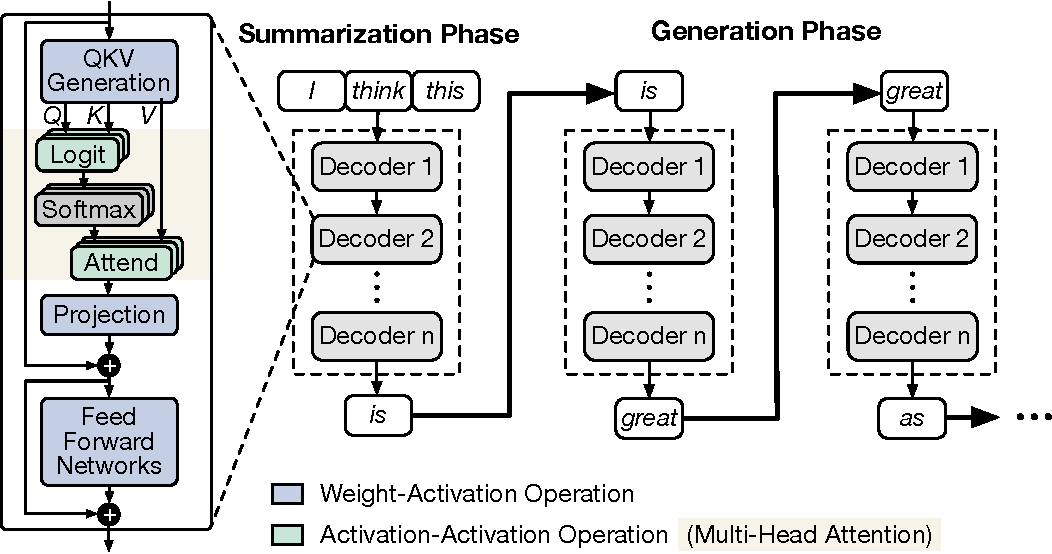
\includegraphics[width=1.0\linewidth]{figure/fig2-gpt-phases.pdf}
\vspace{-4ex}
\caption{Model architecture and inference in LLMs.}
\vspace{-2ex}
\label{fig:llm-inference}
\end{figure}

\niparagraph{Model architecture and execution of LLMs.}
%
Figure~\ref{fig:llm-inference} illustrates the model architecture that all state-of-the-art large language models share~\cite{bert:2018, touvron23-llama, zhang22-opt, mpt, google23-palm2, megatronlm}. 
%
This illustration serves as a recurring example throughout the paper.
%
For an input prompt (e.g., "I think this"), the model undergoes an summarization phase, encoding the input to establish context for the subsequent generation phase.
%
In the generation phase, the model produces tokens one at each iteration in an autoregressive manner, using the generated key-value projections for the next iteration.
%
Both phases constitute a sequence of decoder blocks, each comprising three major layers: (1) QKV generation, (2) multi-head attention (MHA), and (3) a set of feed-forward networks (FFNs).

\begin{figure}[t]
\centering
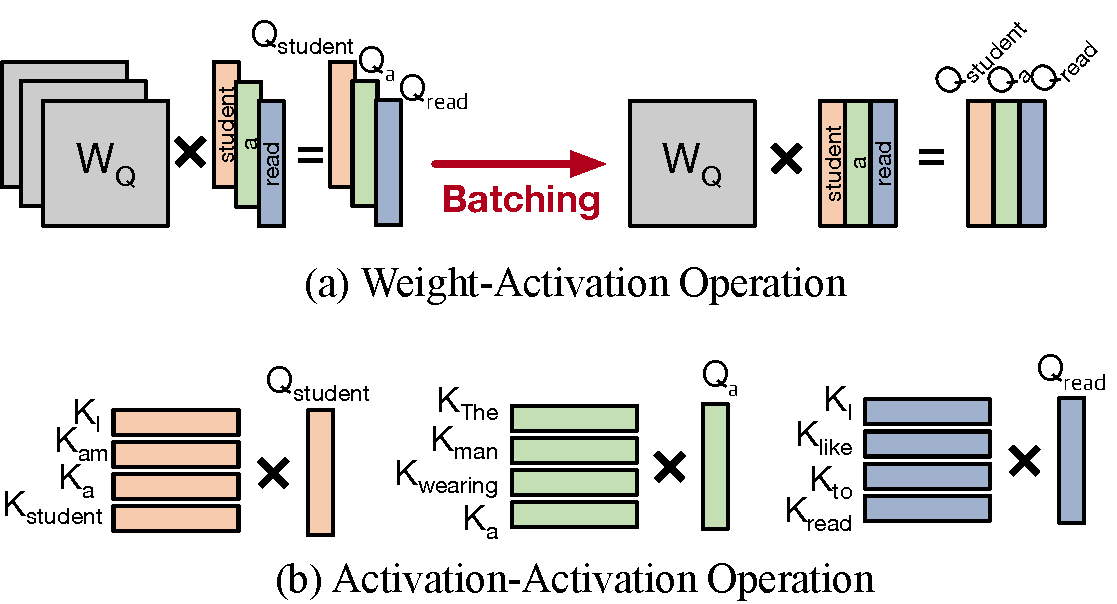
\includegraphics[width=0.9\linewidth]{figure/fig3-batching.pdf}
\vspace{-3ex}
\caption{Operators in a LLM decoder block.}
\vspace{-2ex}
\label{fig:llm-batching}
\end{figure}

\niparagraph{Batched inference of LLMs.}
%
Computationally, the MHA layers have significantly different characteristics than QKV generation and FFN layers. 
%
Figure~\ref{fig:llm-batching} denotes the example tensor operations of LLMs that show (a) weight-activation multiplications, and (b) activation-activation multiplications. 
%
The computations for QKV generation and FFNs are performed by multiplying a per-token Q/K/V activation or attention vector with the trained weight matrices (GEMV). 
%
However, these GEMV operators are transformed into GEMMs when (1) they are located at the decoders in the summarization phase, getting multiple token vectors in parallel (e.g., ``I think this'') or (2) multiple inferences are batched, further parallelizing the computations for multiple single-token generation processes. 
%
On the other hand, the computations for MHA layers are multiplications between two different activations where one is for the current token (vector), and the other is for all the tokens before the current token (matrix), rendering a matrix-vector multiplication (GEMV). 
%
As the activation operands are unique for each inference request, their batching is not possible, making the computations highly memory bandwidth-bound.  
%




\niparagraph{Analysis of arithmetic intensity.}
%
To better understand the computational characteristics of LLM inference, we conduct a roofline analysis using two GPT3 variants, GPT3-13B and GPT3-175B. 
%
Figure~\ref{fig:arithmetic-intensity} shows the relationship between the arithmetic intensity (FLOPS/byte) and performance (TFLOPS).
%
We observe that for both models, the generation phases are severely memory-bound, while the summarization phases are compute-bound.
%
As these two phases have algorithmic dependencies and occur alternately in a sequential manner, it is fundamentally challenging to achieve high resource utilization using a homogeneous computing platform.   
%
This insight motivates this work and drives us to design a heterogeneous system that combines a compute-centric systolic array-based NPU for GEMMs with memory-centric Processing-in-Memory (PIM) accelerators for GEMVs.


\begin{figure}[t]
\centering
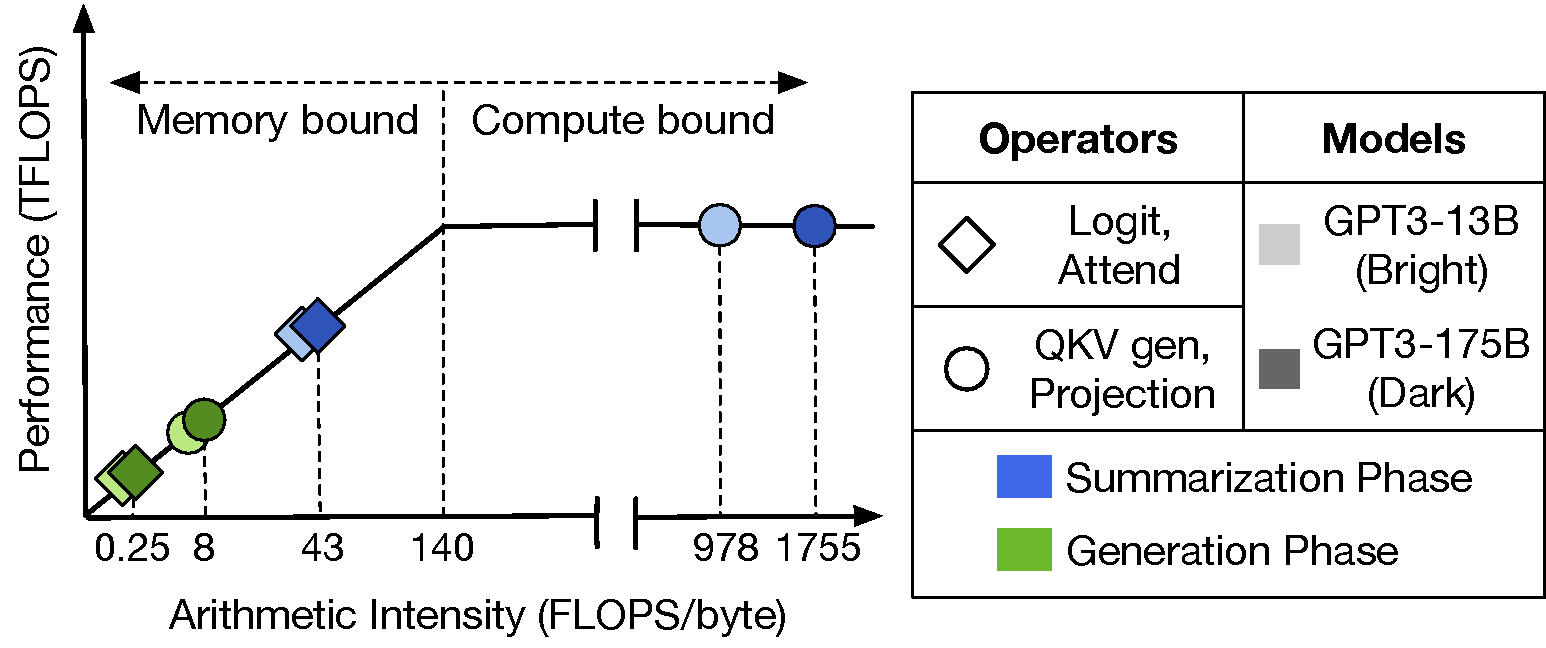
\includegraphics[width=1.0\linewidth]{figure/fig4-arithmetic-intensity.pdf}
\vspace{-4ex}
\caption{Arithmetic intensities of LLM layers.}
\label{fig:arithmetic-intensity}
\vspace{-3ex}
\end{figure}


\subsection{LLM Inference Serving}
%
As there is a massive resource demand for LLMs, the de-facto practice is to build large-scale inference serving frameworks such as DeepSpeed~\cite{deepspeed}, Orca~\cite{orca} and vLLM~\cite{vllm}.
%
These frameworks offer inference services for customer requests (i.e., prompts), which enables batching.
%

\niparagraph{Selective batching.}
%
In general, batching is an effective method for neural network inference to improve resource utilization, while not sacrificing the latency requirement.
%
However, MHA layers pose a challenge as they do not allow batching. 
%
This presents a difficulty for hyperscalers dealing with numerous customer requests while operating within limited compute resources.
%
To address this, a recent work, Orca~\cite{orca}, proposes a solution where attention layers are individually computed, while QKV generation and FFN layers are batched. 
%
This approach allows the system to still benefit from batching when possible; otherwise, it serializes the computation.
%
This unique algorithmic property necessitates the simultaneous computations of GEMM and GEMV, which is the main motivation for this work.
%

\niparagraph{Iteration level scheduling.}
%
Inference serving system receives requests in a streaming fashion without a deterministic schedule. 
%
Therefore, there is a need for a parallelization approach that can efficiently process the non-deterministically collected set of inference requests.
%
Orca~\cite{orca} additionally proposes to schedule batched inference at the beginning of every iteration. 
%
This allows new inference requests to be added to and terminated requests to be removed from the batch. 
%
Consequently, newly arrived requests do not need to wait until the generation phase for an already-started batch is terminated.
%
This approach can significantly reduce the average latency for inference serving.
%
\neupims is built upon this scheduling technique, and thus, it manages the inference requests at the iteration boundaries. 

%
\niparagraph{Memory paging for attention.} 
%
vLLM~\cite{vllm} is another recent effort to enhance the resource utilization of LLM inference serving systems, with a specific focus on memory management.
%
As discussed in Section~\ref{sec:llm-background}, the QKV generation layer produces KV cache, the input for the attention layers that can be reused in the generation phases. 
%
Leveraging this opportunity, LLM inference systems \emph{cache} the KV projections in the memory, the size of which can be significant when the sequence length becomes large. 
%
vLLM introduces memory paging for this cached data, ensuring that a significant amount of memory is not pre-allocated long before its actual use.
%
\neupims employs the vLLM's paging technique, implementing the page-based memory allocation mechanism for KV cache, which effectively increases the batch size significantly. 

\emph{It is worthwhile to note that \neupims is designed to be deployed on an inference serving system that incorporates all of these aforementioned techniques.}
